\section{Workflow}
\label{chap:workflow}

\subsection{Methodology}
The project is going to us the \textbf{Kanban} agile methodology, and \textbf{Jira} to manage the project. I chose agile against waterfall because it makes it easier to continue the project once ended and it's also easier to share the tasks with the open-source community. I also considered using Scrum, but because I'm going to be the only active developer it would add a lot of overhead to the management, so with Kanban, I'll be able to develop faster.

\vspace*{\fill}
\begin{figure}[ht!]
    \center
    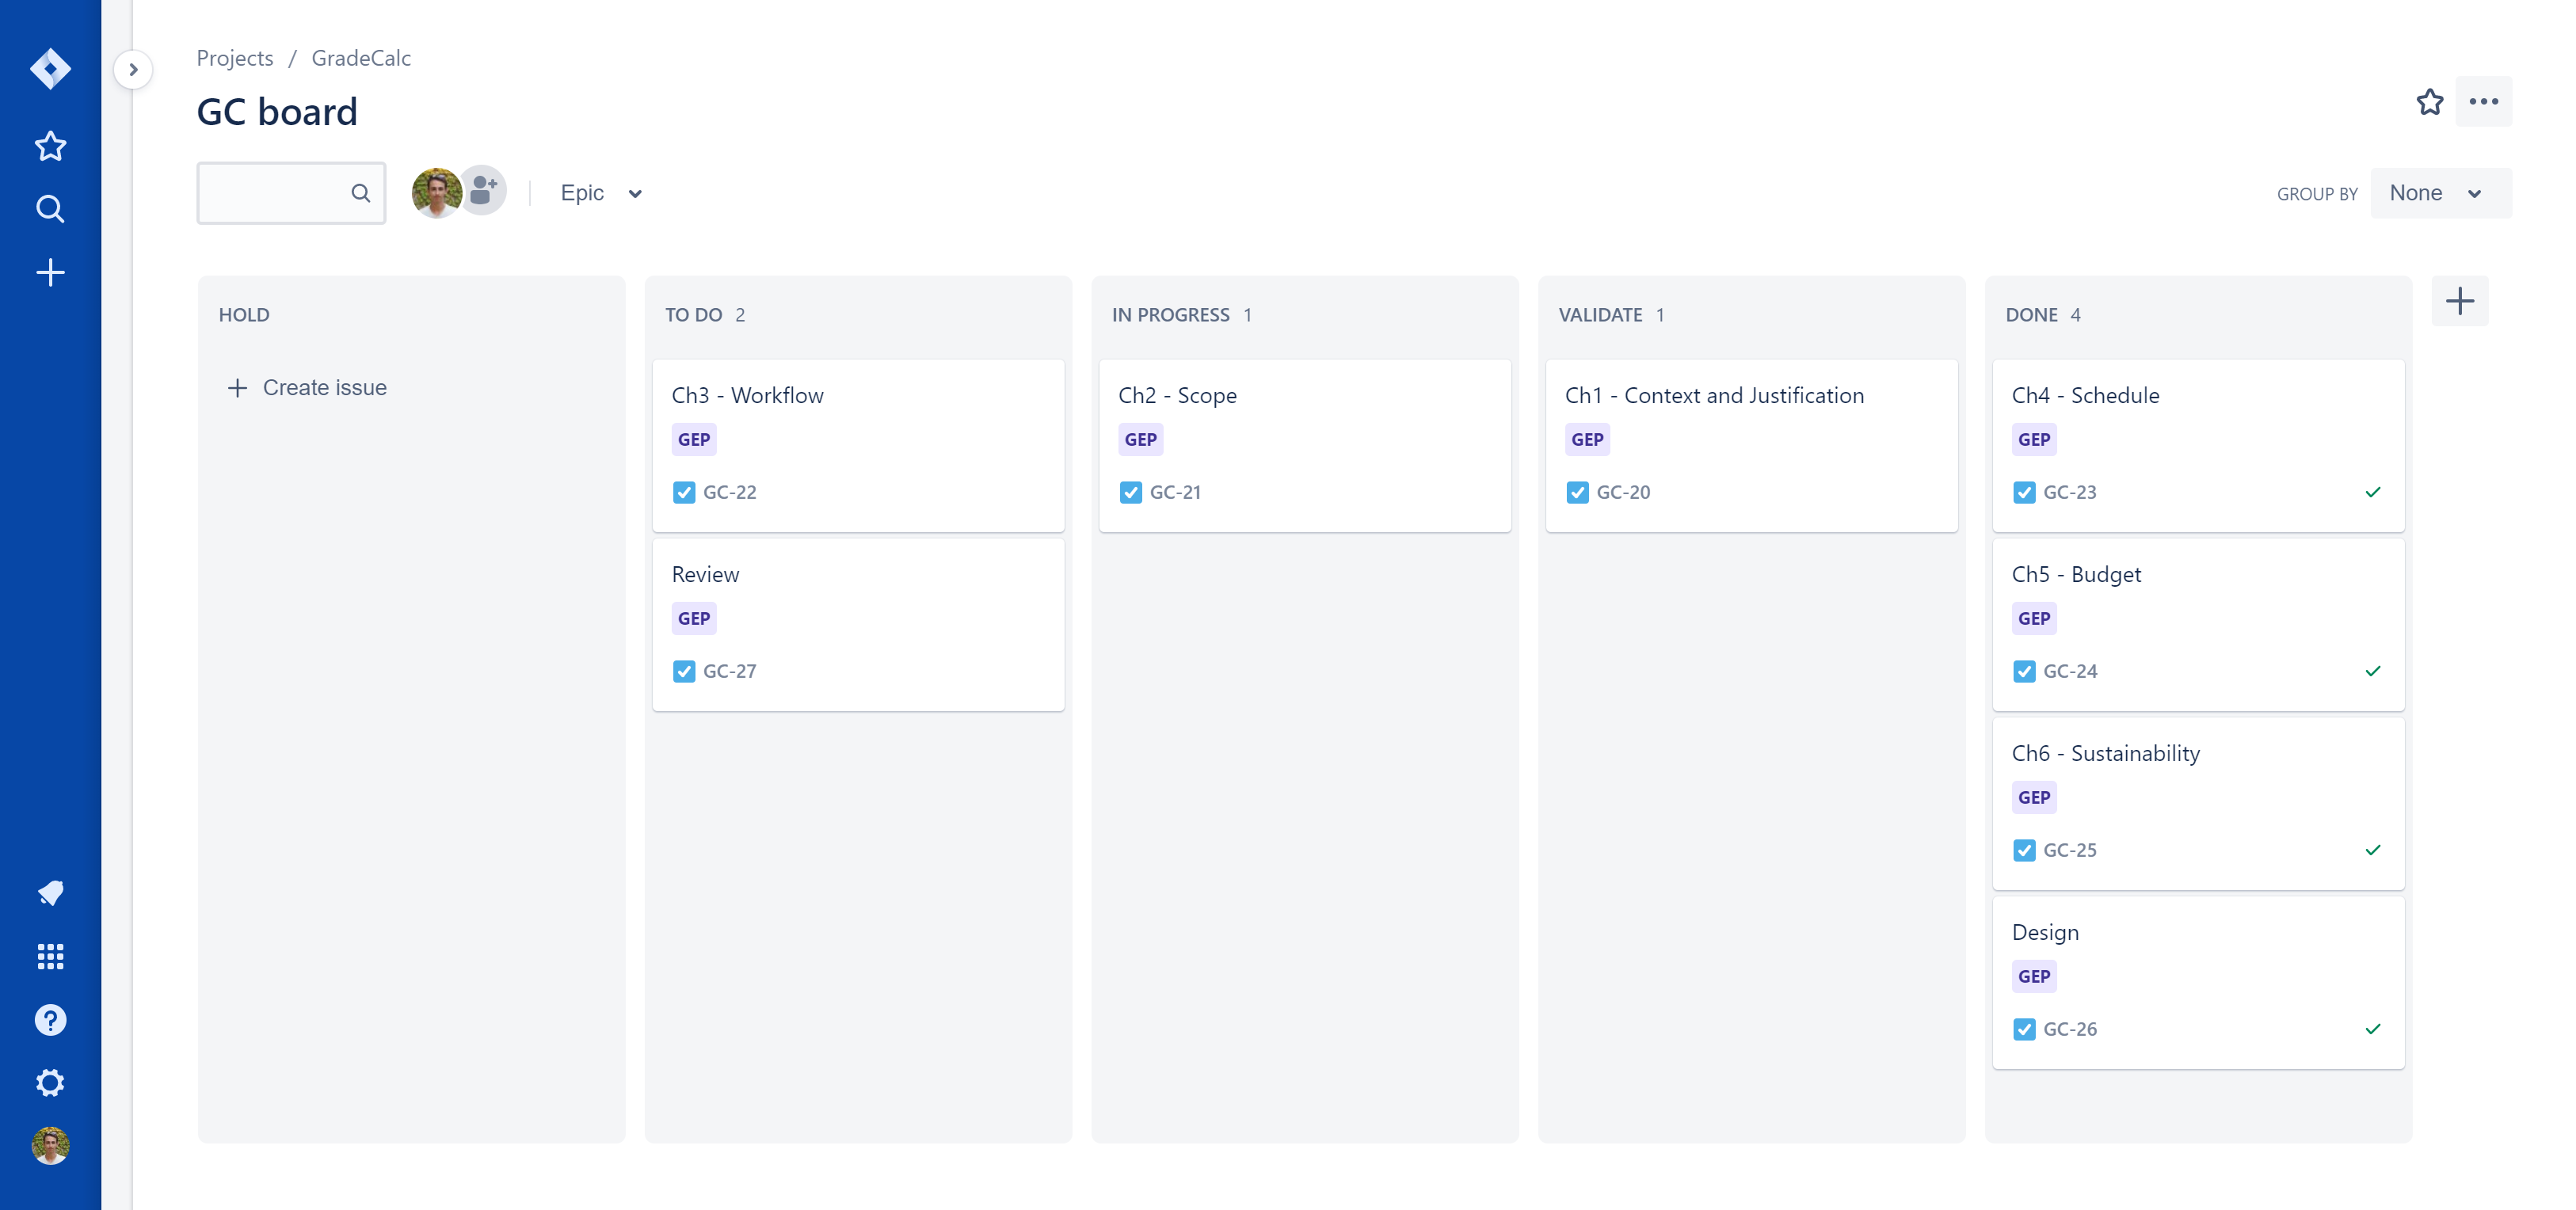
\includegraphics[width=1\columnwidth,frame]{media/jira-board-gep.png}
    \caption[Kanban board in Jira]{Kanban board in Jira (\url{https://mauriciabad.atlassian.net/browse/GC})}
    \label{jira-board-gep}
\end{figure}
\vspace*{\fill}

\newpage
The Kanban board is going to have the following columns:
\begin{itemize}
    \item \textbf{HOLD}: Defined tasks that don't have to be done yet. Usually due to dependencies or external factors.
    \item \textbf{TO DO}: Tasks to do once there's room in the IN PROGRESS column.
    \item \textbf{IN PROGRESS}: Tasks being performed at the moment.
    \item \textbf{VALIDATE}: Apparently finished tasks that need to be tested and validated. If it's not right, it will be moved back to IN PROGRESS.
    \item \textbf{DONE}: Finished and validated tasks.
\end{itemize}

The DONE tasks are going to be removed from the Kanban to the backlog at the end of each sprint, and tasks from the backlog moved to the Kanban HOLD column.

The project is going to use GitHub Flow \cite{github-flow}, a lightweight branch-based workflow. It's specially crafted for Continuous Integration apps and reduces overhead to the minimum. In addition, most open-source projects adopt it.
\vspace*{\fill}
\begin{figure}[ht!]
    \center
    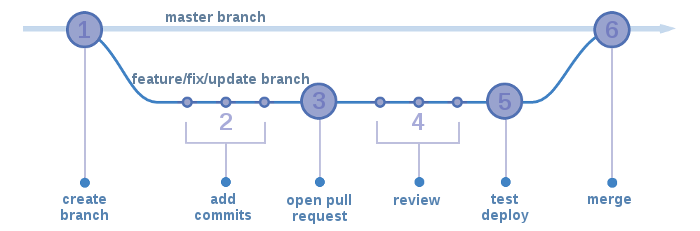
\includegraphics[width=1\columnwidth]{media/github-flow.png}
    \caption[GitHub Flow]{GitHub Flow \cite{github-flow}}
    \label{github-flow}
\end{figure}
\vspace*{\fill}

\newpage
\subsection{Tools}
To manage the project and validate that tasks are indeed completed, the following tools are going to be used:
\begin{itemize}
    \item \textbf{GitHub}: Version control system and issue tracker.
    \item \textbf{Jira}: Project management tool.
    \item \textbf{Netlify}: Continuous deployment.
    \item \textbf{Travis CI}: Continuous integration it runs all tests.
    \begin{itemize}
        \item \textbf{Jest}: Testing framework.
        \item \textbf{Lighthouse}: Audits performance, accessibility, PWA\footnote{Progressive Web App}, SEO\footnote{Search Engine Optimization} and more.
    \end{itemize}
\end{itemize}

\vfill
\begin{figure}[h!]
    \center
    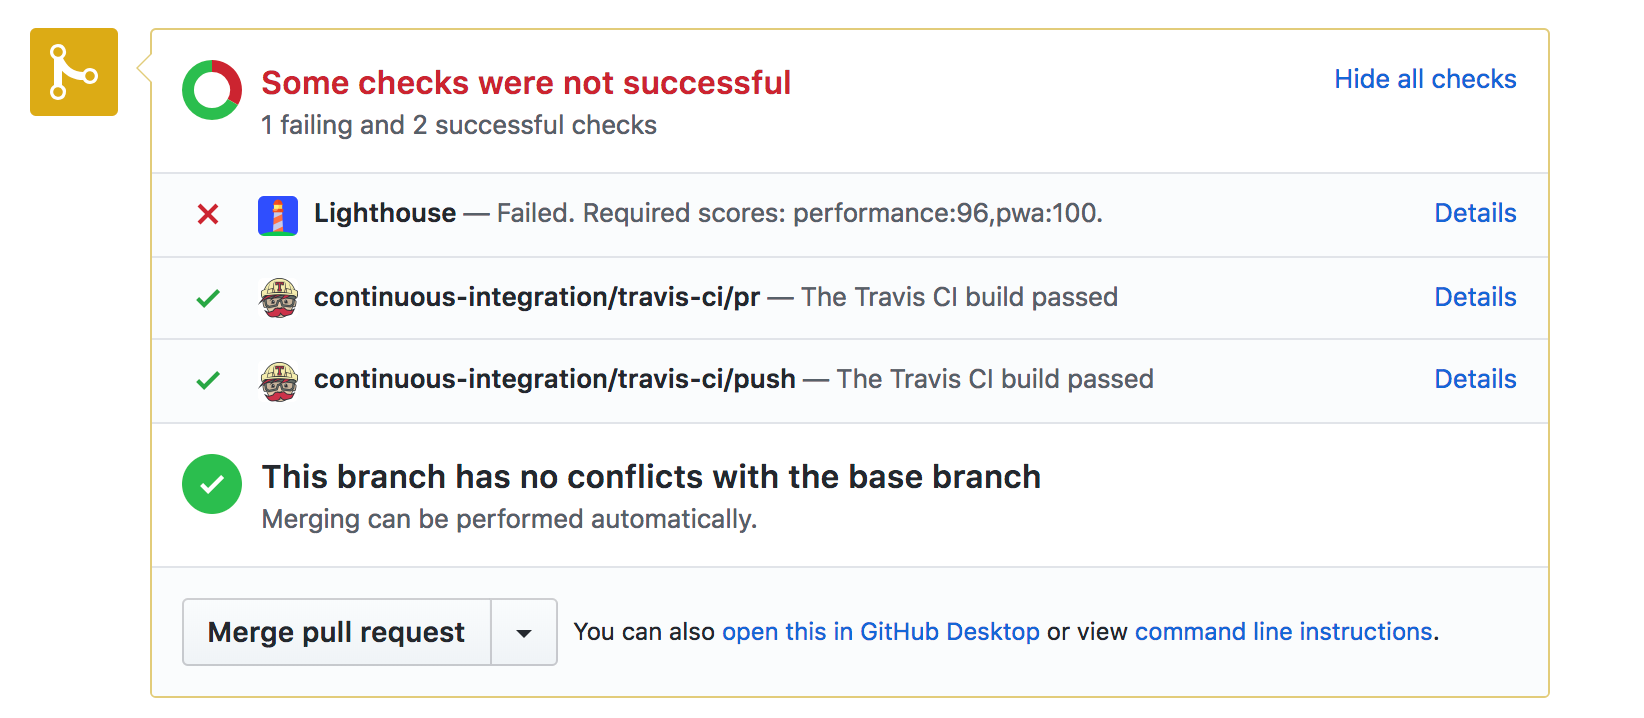
\includegraphics[width=1\columnwidth]{media/github-ci.png}
    \caption[GitHub CI]{GitHub CI - Pull request UI}
    \label{github-ci}
\end{figure}
\vfill

\newpage
\subsection{Changes in the workflow}

The workflow established at the beginning of the project (chapter \ref{chap:workflow}) has been followed but not in a strict way. No main changes have been made.

Jira ended up not being used. At the beginning I used it, but I ended up having a to-do list in a markdown text file and just checking the checkboxes once done. 

This change was made because Jira was slowing down productivity. I had to fill in many fields when creating and editing the issues. In contrast, a simple checklist has no overhead at all. 

The typical problem of using a to-do list is that when there are many tasks there's a lack of order and teamwork becomes hard. Because this project doesn't have many tasks and there are almost no dependencies between them using a to-do didn't introduce any problem, simplifying a lot the project management. 

And, of course, if the project scales in the future and a to-do list becomes an obstacle, a tool like Jira will become again the standard to manage it.
